% !TEX root = paper.tex

\section {Results}
\label{sec:results}

\subsection{Ridge yield}

\begin{figure}[h!]
	\centering
	\subfigure{ 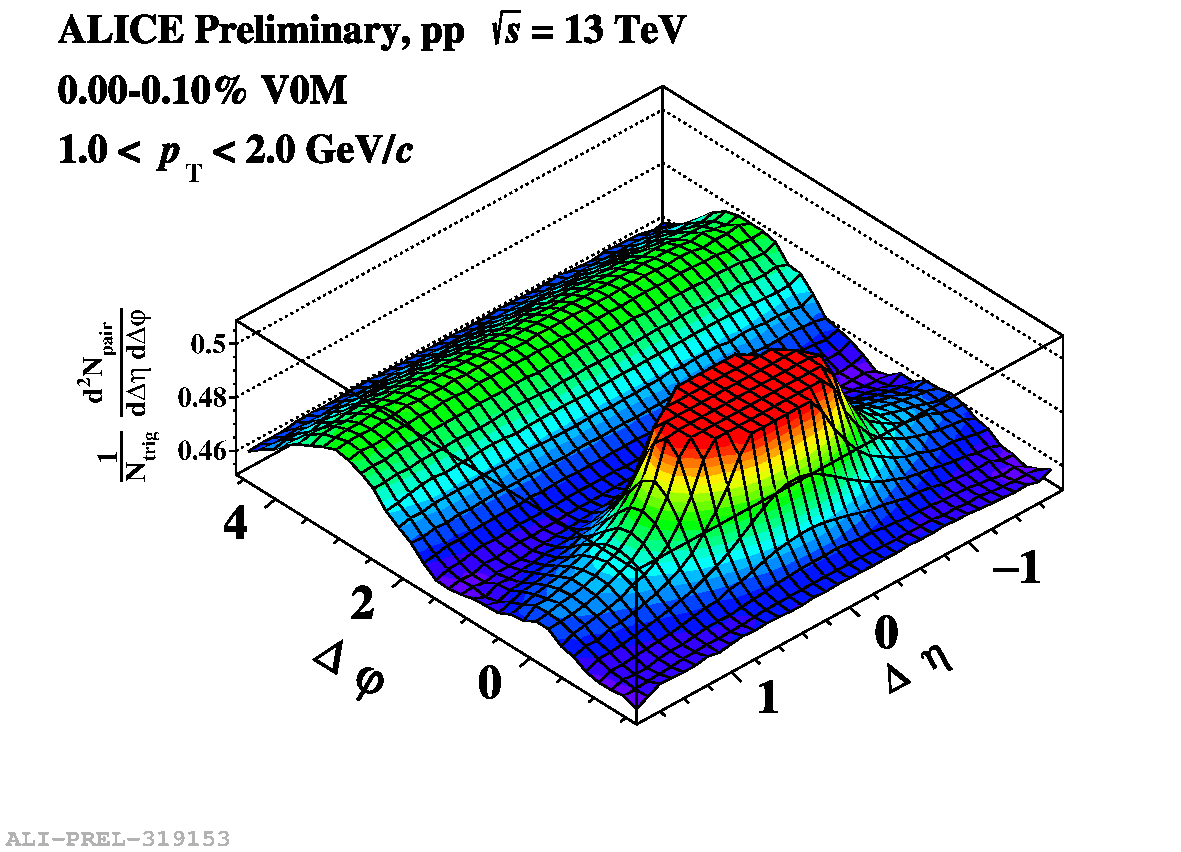
\includegraphics[width=0.47 \textwidth]{./figures/corr1.pdf} }
	\subfigure{ 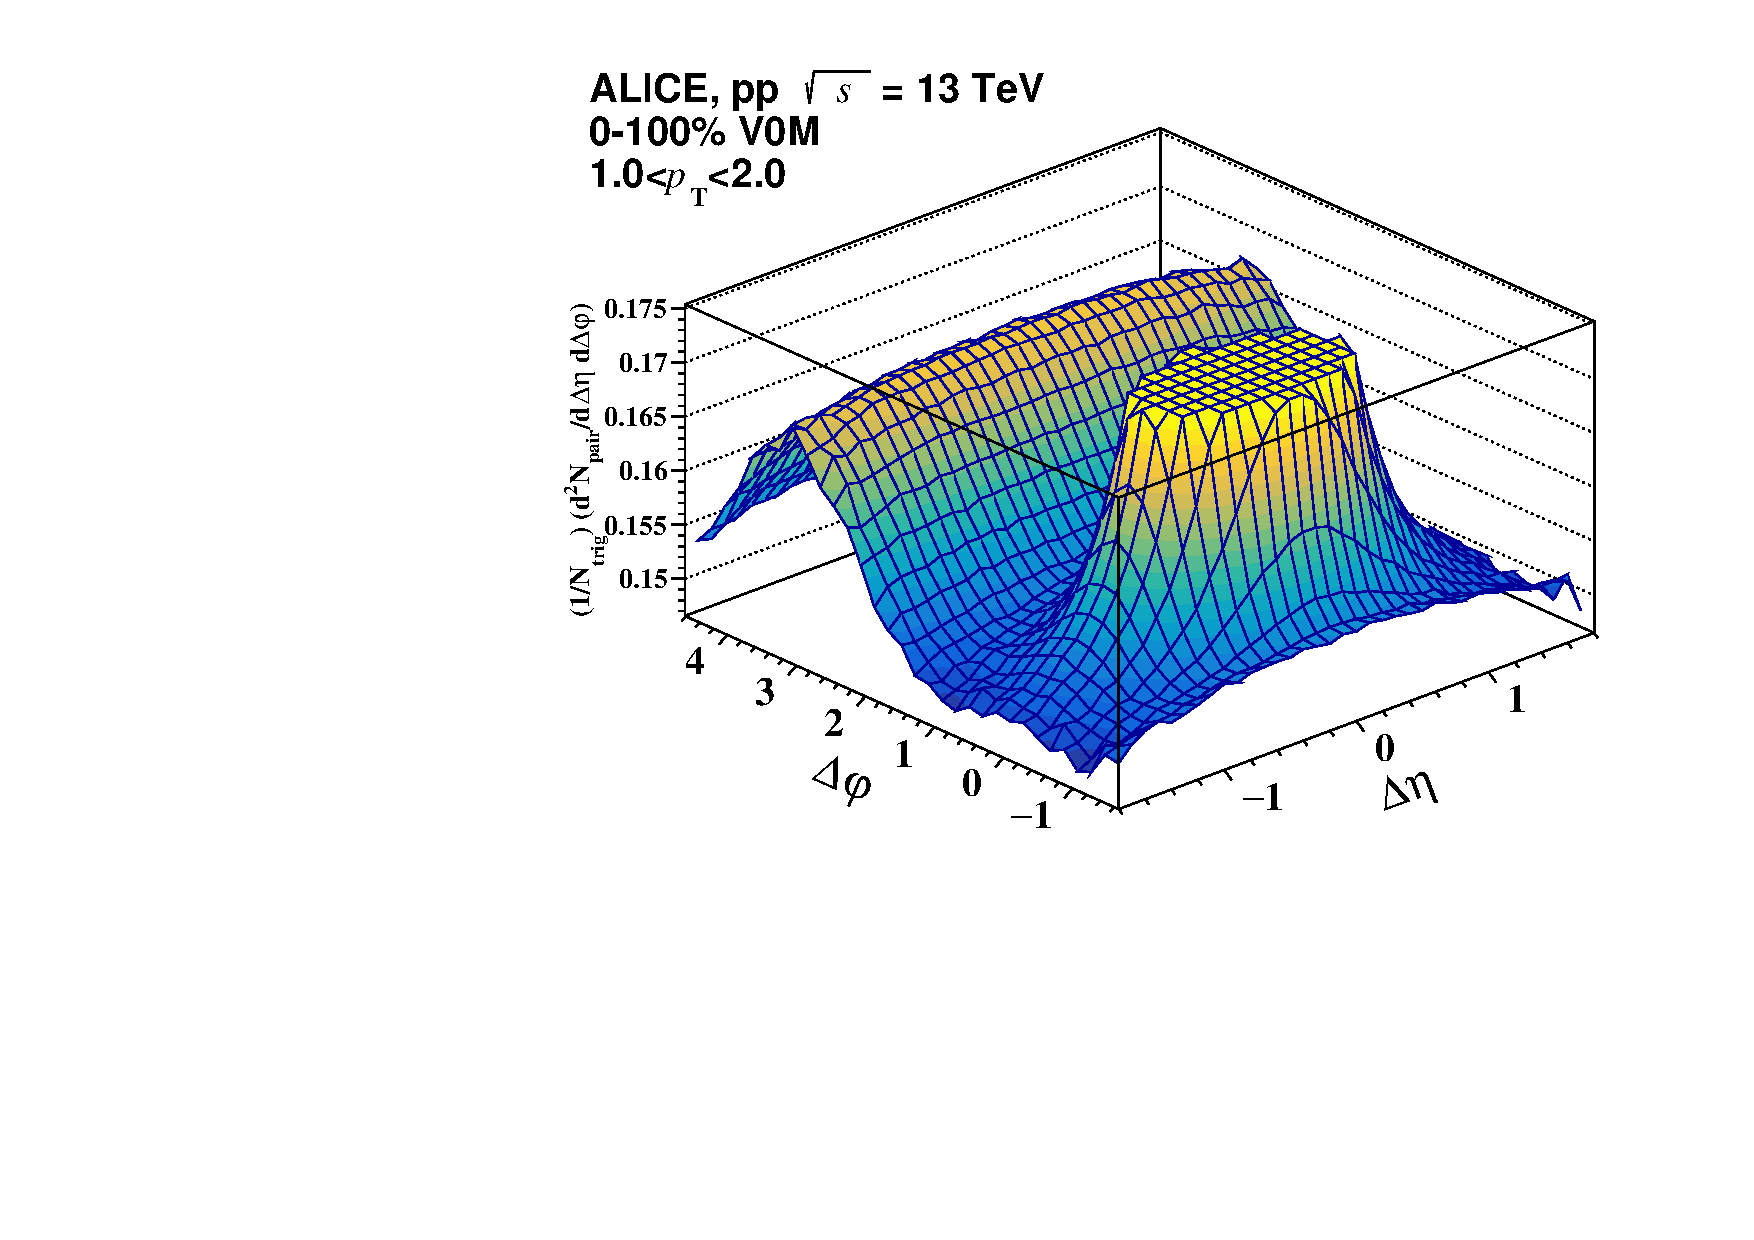
\includegraphics[width=0.47 \textwidth]{./figures/corrmb.pdf} }
	\caption{ Dihadron correlation functions as functions of $\Delta\eta$ and $\Delta\varphi$ in high-multiplicity (0--0.1\%, left) and minimum-bias events (0--100\%, right). The intervals of $\pttrig$ and $\ptassoc$ are equally $1 < \it{p}_{\rm{T}} < $2 GeV/$c$. }
	\label{fig:PlotCorrMBHMT}
\end{figure}

Figure~\ref{fig:PlotCorrMBHMT} shows two-particle correlation functions as a function of the $\Delta \eta$ and $\Delta \varphi$ separation of trigger and associated particles. The per trigger yield is measured with Eq.~\ref{eq:corrfunction} for $1 < \pttrig~\mathrm (\ptassoc) < $2 GeV/$c$ in pp collisions at $\sqrt{\it{s}} = $\unit{13} {\rm{}TeV}. The left panel is for the high-multiplicity class. The right one is from the minimum bias events. The ridge structure is clearly observed in the high-multiplicity class while it is less visible and conclusive in the minimum bias events. The away-side yield is populated mostly by correlation of jets which are back-to-back.

\begin{figure}[h!]
	\centering
	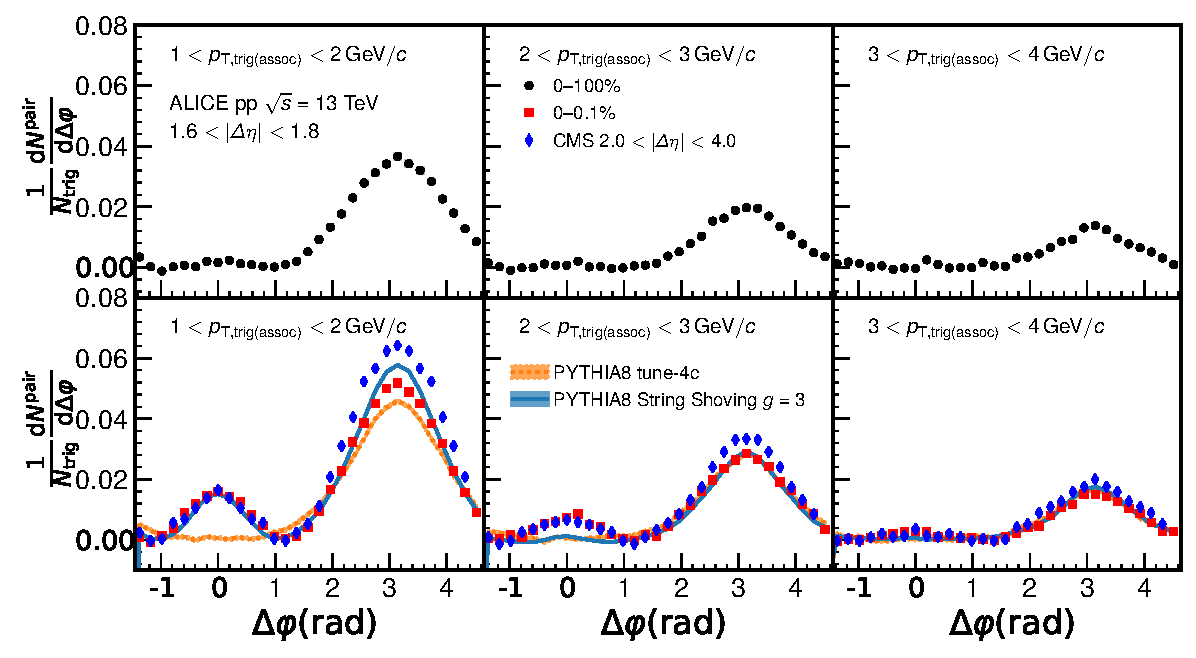
\includegraphics[width=0.9\linewidth]{./figures/Fig2_PlotDeltaPhi.pdf}
	\caption{One-dimensional $\Delta\varphi$ distribution in the large $\Delta\eta$ projection for three transverse momentum intervals in high-multiplicity and minimum bias events. The distributions in upper panels are measured with 0--100\% multiplicity class. The distribution in lower panels are measured with 0--0.1\% multiplicity class. Transverse momentum ranges of trigger particle and associated particle are $1<\pt<$2 (left), 2$<\pt<$3 (middle) and 3$<\pt<$4 GeV/$c$ (right), respectively. The model predictions are presented using $\pythiashoving$, $\pythiam$, and $\epos$.}
	\label{fig:PlotDeltaPhi}
\end{figure}
 
Projected $\Delta\varphi$ distributions of the two-particle correlation functions in $1.6<|\Delta\eta|<1.8$ are shown in Fig.~\ref{fig:PlotDeltaPhi} for various $\it{p}_{\rm{T}}$ intervals in the minimum bias class and the high-multiplicity class down to 1 GeV/$c$ where non-flow contamination is negligible. The near-side ($\Delta\varphi\sim 0$) ridge in high-multiplicity class is clearly observed in all transverse momentum ranges studied while there is no hint of the signal in the minimum bias class. Within the range of analyzed particle $\pt$, yield in the near-side ridge decreases with increasing $\pt$ in the high-multiplicity class. The measurements in the high-multiplicity class are compared to the results published by the CMS collaboration~\cite{Khachatryan:2015lva}. In case of the CMS measurement, charged particle multiplicity was obtained by counting $\pt>0.4$ GeV/$c$ tracks in $|\eta|<$2.4. In our analysis, event multiplicity is determined from the forward V0 detectors. The difference of multiplicity definition between the ALICE and the CMS was studied based on Pythia8 event generator. The mid-rapidity particle distributions are extrapolated using 0--0.1\% event defined by V0M. CMS acceptance for counting multiplicity was applied to the extrapolated particle distribution. The multiplicity from the distribution is 96, which is about 20\% lower than the multiplicity the CMS used. %By interpolating the $\eta$ and $\pt$ distributions based on PYTHIA, it is found that the multiplicity in \cite{Khachatryan:2015lva} is about 20\% higher than 0--0.1\% in this analysis, corresponding 0--0.03\%. 
Near-side ridges in all transverse momentum ranges are comparable to each other within the uncertainties. The larger away yields observed in \cite{Khachatryan:2015lva} can be attributed to the difference in jet acceptance in $\eta$. The ALICE data are compared with model predictions where we apply the comparable high-multiplicity selection and $\Delta\eta$ projection range. The high-multiplicity class for each model is determined by requiring the minimum number of charged particles larger than 105 in the V0M acceptance, which corresponds to the top 0--0.1\% multiplicity class based on $\pythiam$, where 110 and 108 are corresponding multiplicities for $\epos$ and $\pythiashoving$, respectively. The $\pythiashoving$ gives good estimates of the near-side ridge yield and slightly overestimates the away-side yield for the interval of 1$<\it{p}_{\rm{T}}<$2 GeV/$c$. However, the $\pythiashoving$ underestimates the near-side ridge yield for the $\it{p}_{\rm{T}}>$2 GeV/$c$ range. $\pythiam$ does not show any peaks in the near-side as expected. It slightly underestimates the away-side peak for $1<\it{p}_{\rm{T}}<$2 GeV/$c$ and gives good estimates for the $\it{p}_{\rm{T}}>$2 GeV/$c$ range. On the other hand, $\epos$ describes quantitatively better the $\pt$ dependence in the 1$<\it{p}_{\rm{T}}<$4 GeV/$c$ range, while overestimating the near-side ridge yield for the $\it{p}_{\rm{T}}<$2 GeV/$c$ range. 


\begin{figure}[h!]
	\centering
	\subfigure{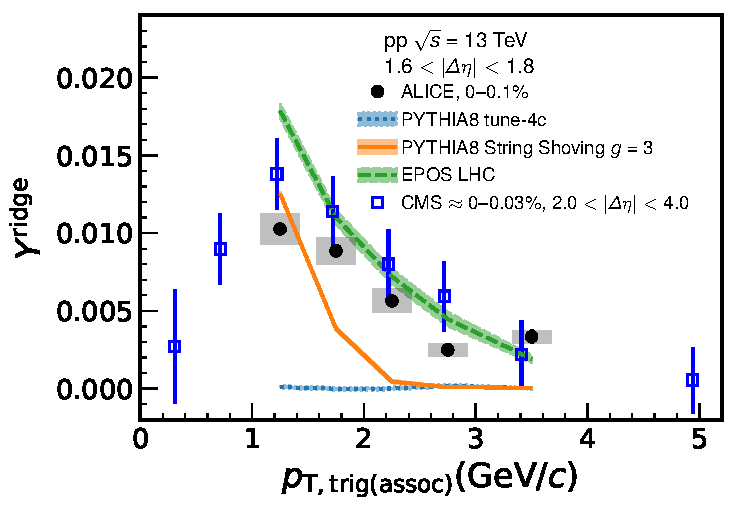
\includegraphics[width=0.99\textwidth]{./figures/Fig3_PlotRidgeYield.pdf}}
	\caption{ Fully corrected near-side ridge yield as a function transverse momentum. The filled circles denote the measurement with ALICE. The CMS measurement~\cite{Khachatryan:2015lva} is represented by open blue box markers. The three lines show model predictions from $\pythiam$ (blue line), $\pythiashoving$ (orange line) and $\epos$ (green line).}
	\label{fig:PlotYSpect}
\end{figure}

Fig.~\ref{fig:PlotYSpect} shows the near-side ridge yield measured in high-multiplicity events as a function of transverse momentum. The ALICE data are compared to \cite{Khachatryan:2015lva}.
%The ridge yields as a function of the transverse momentum are shown in Fig.~\ref{fig:PlotYSpect} in the high-multiplicity class and compared to \cite{Khachatryan:2015lva}.
Taking into account the differences in acceptance of charged tracks and estimated multiplicity, the slight disagreement between the two sets of results could be expected. The spectrum is also compared with model calculations. $\pythiam$ gives zero yields since it does not contain the ridge effect. $\pythiashoving$ describes the yield qualitatively however the predicted yield decreases more rapidly than the measured one as $\pttrigassoc$ increases. $\epos$, unlike $\pythiashoving$, describes well the $\pt$ dependence of the ridge yield for the $\it{p}_{\rm{T}}>$2 GeV/$c$ range, while predicting larger yield for $\it{p}_{\rm{T}}<$2 GeV/$c$.

\subsection{Event-scale dependence of the ridge yield}
\begin{figure}[h!]
	\centering
	\subfigure{ 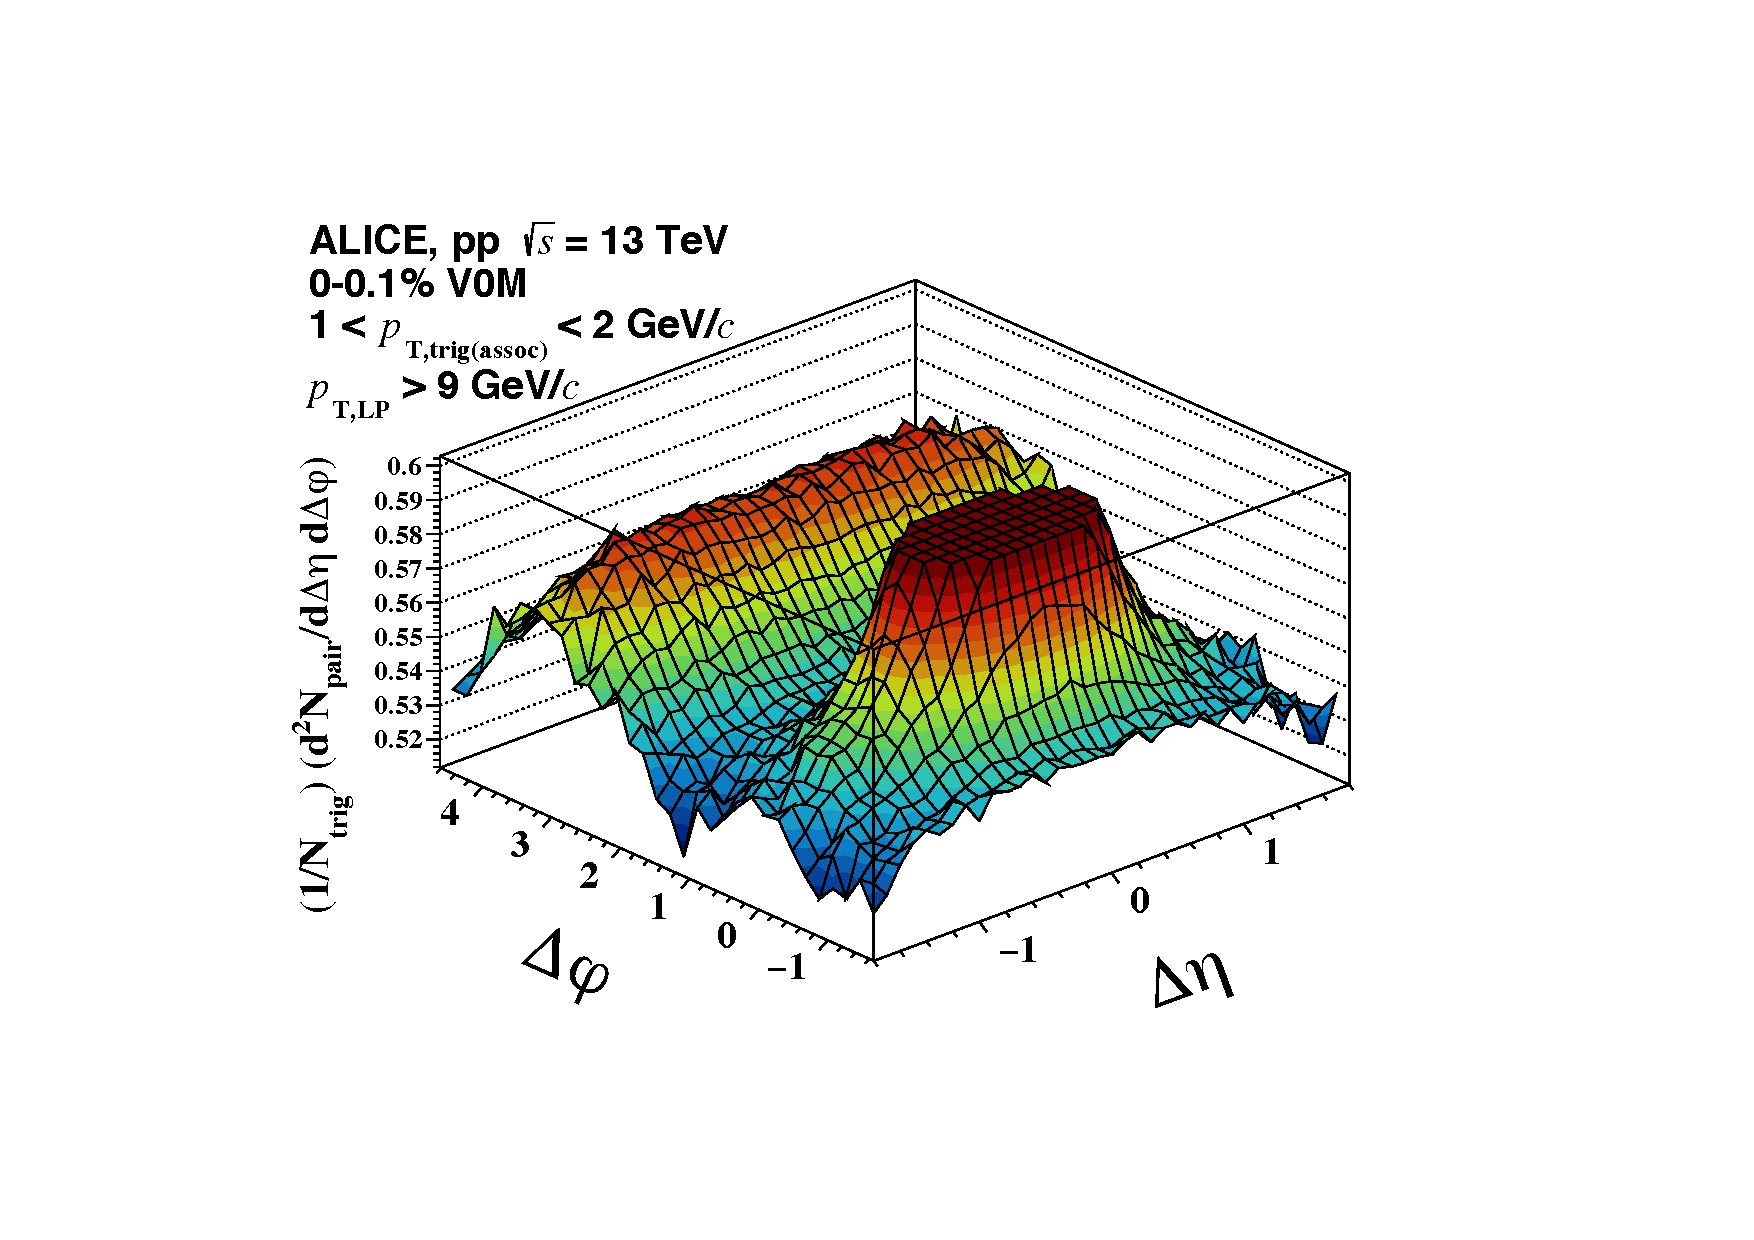
\includegraphics[width=0.47 \textwidth]{./figures/corrlh.pdf} }
	\subfigure{ 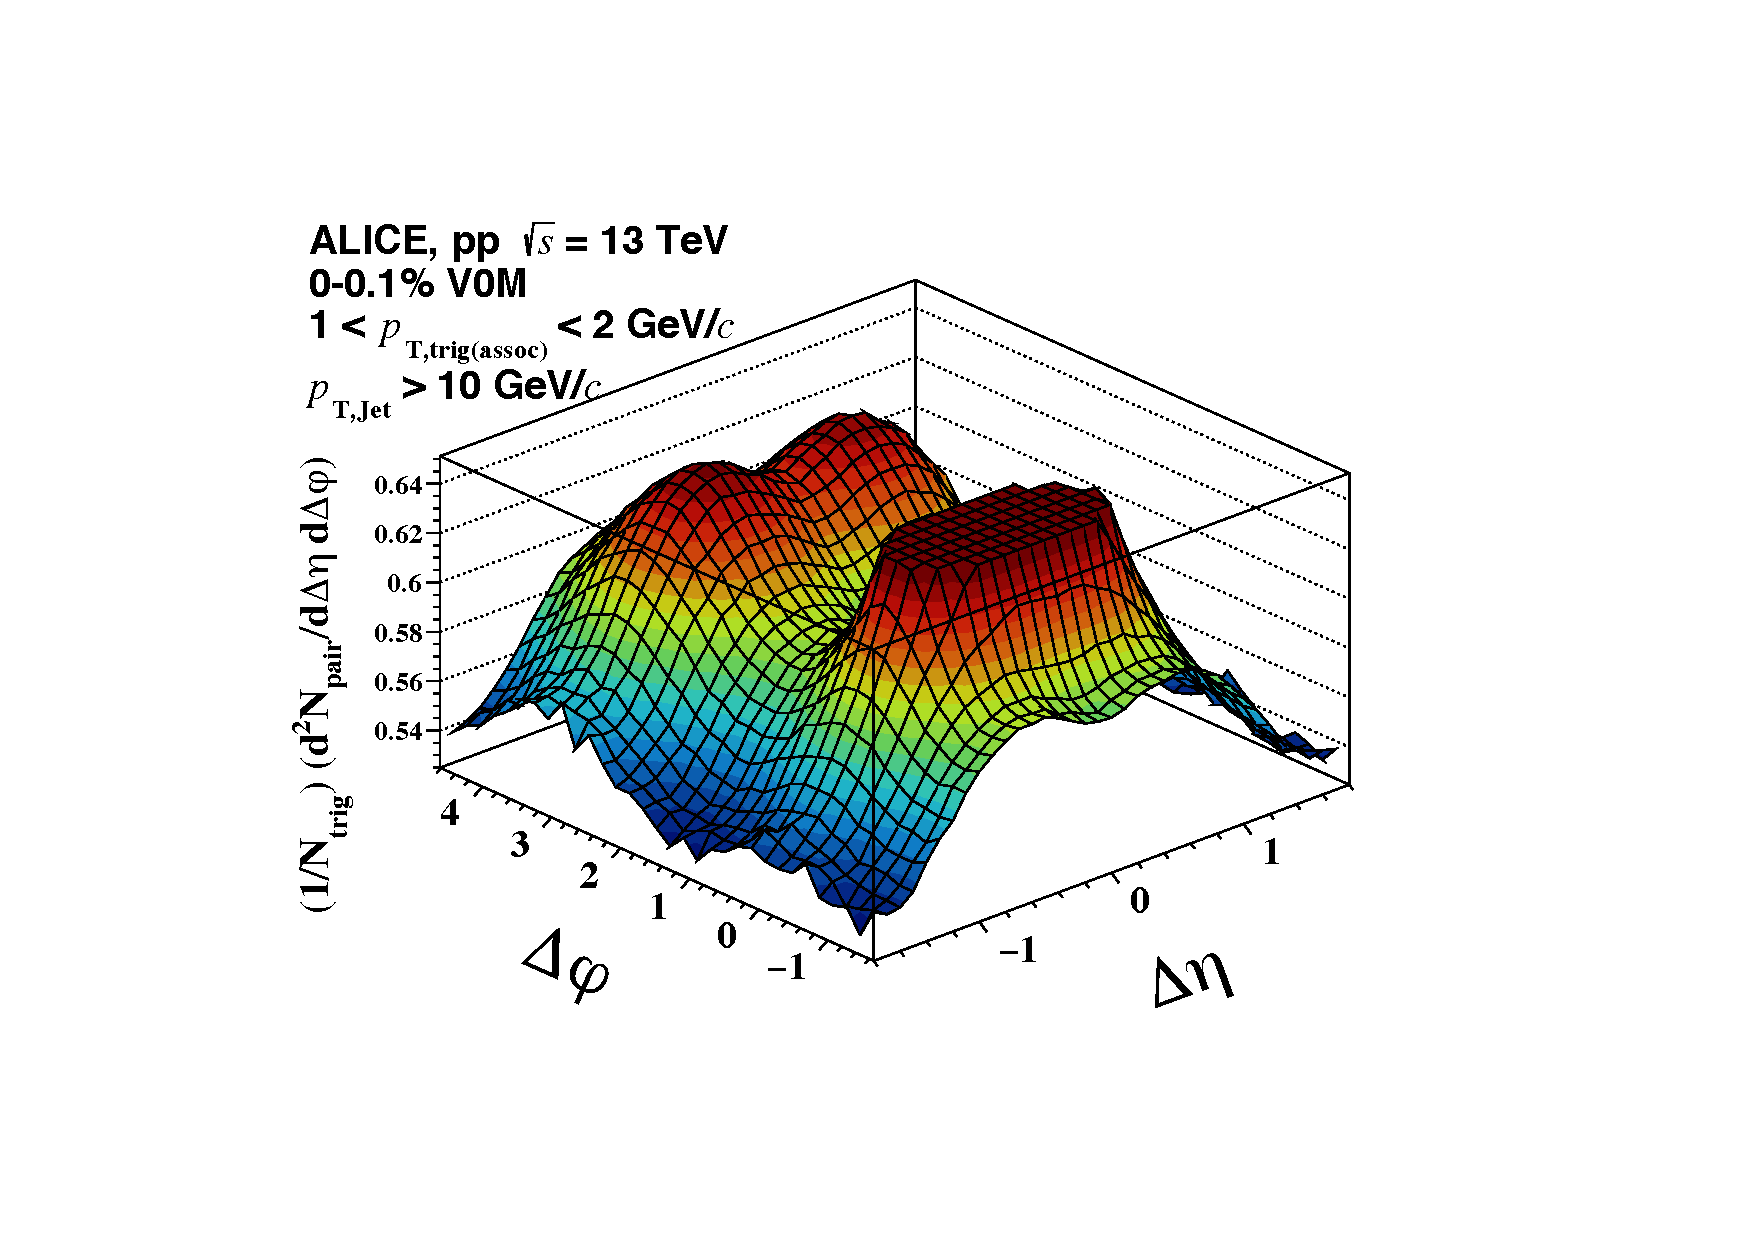
\includegraphics[width=0.47 \textwidth]{./figures/corrjet.pdf} }
	\caption{ Two-dimensional correlations function as a function of $\Delta\eta$ and $\Delta\varphi$ in thigh-multiplicity events where a selection on event-scale was required in addition. The interval of $\pttrig$ and $\ptassoc$ is 1$<\pt<$2 GeV/$c$. Left: selecting HM events with a $\ptlead>$ 9 GeV/$c$ leading track. Right: selecting HM events with a $\ptlead>$ 10 GeV/$c$}
	\label{fig:PlotCorrHMTSel}
\end{figure}

The ridge yield is further studied with respect to two different event-scales. In the first measurement, the event-scale is set by requiring a minimum $\pt$ cutoff on a leading track in event (denoted as $\ptlead$), while in the second measurement, we impose a minimum $\pt$ cutoff on a leading jet  (denoted as $\ptjet$). As shown in Fig.~\ref{fig:PlotCorrHMTSel}, the ridge structure for $1< \pttrig\,(\ptassoc) <2$ GeV/$c$ still persists in high-multiplicity pp collisions with $\ptlead>9$~GeV/$c$ (left) and $\ptjet>10$~GeV/$c$ (right) .  %The interval is the same to the measured ridge yield is maximum without the event-scale selection.
It is worth noting that the correlation function with the minimum $\ptjet$ selection has a double peak structure which is oriented along $\Delta\eta$ axis at $\Delta\varphi=\pi$. This structure emerges due to jet tagging within the limited acceptance in mid-rapidity.

\begin{figure}[h!]
	\centering
	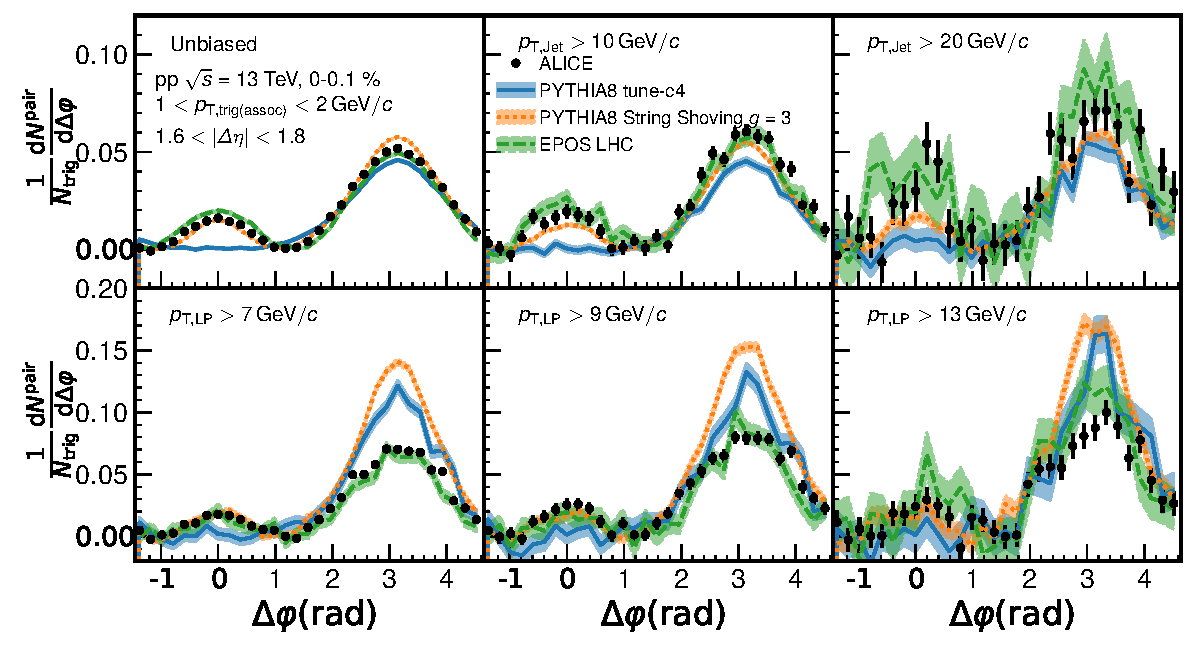
\includegraphics[width=0.99\linewidth]{./figures/Fig5_PlotDeltaPhiESE.pdf}
	\caption{ $\Delta\varphi$ projections of the correlation function constrained to 1.6$<|\Delta\eta|<$1.8 in HM events with additional event-scale bias. Top: imposing a cut on leading jet,  bottom: imposing a cut on leading hadron. ALICE data are compared with prediction of models.}
	\label{fig:PlotDeltaPhiESE}
\end{figure}

Figure~\ref{fig:PlotDeltaPhiESE} shows projected $\Delta\varphi$ distributions of the correlation functions in $1.6<|\Delta\eta|<1.8$ with the minimum $\ptlead$ (lower) and $\ptjet$ (upper) requirement. Even with the event-scale selection, the ridge is still visible at the near-side. The near-side ridge peak increases as the thresholds of $\ptlead$ and $\ptjet$ increase compared to the one measured in unbiased events. The results are compared with $\pythiashoving$, $\pythiam$, and $\epos$ calculations. Near-side ridge peaks are qualitatively reproduced by $\pythiashoving$ and $\epos$. On the other hand, $\pythiam$ does not show the  near-side ridge peak for neither of the two event-scale selection, but it gives compatible results for the away-side yield as $\pythiashoving$.
%Both models describe the away-side yield with the $\ptjet$ selection and overestimate away-side yield with the $\ptlead$ selection.

\begin{figure}[h!]
	\centering
	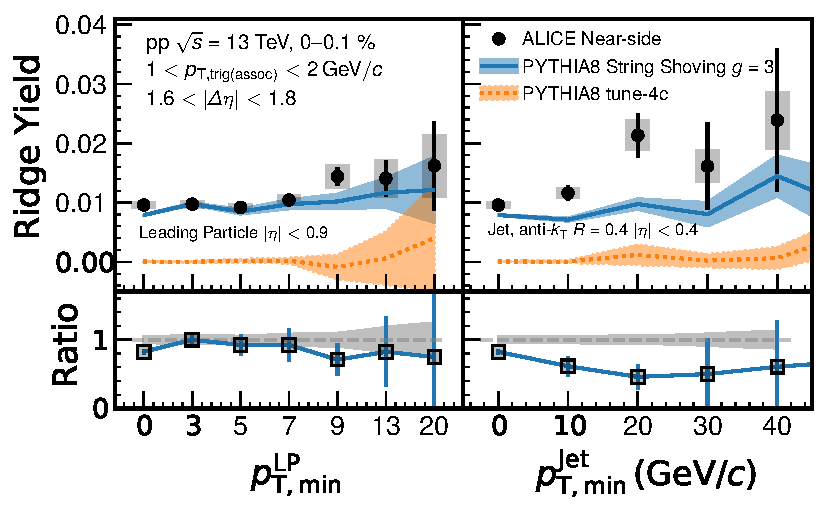
\includegraphics[width=0.89\linewidth]{./figures/Fig6_RidgeYieldESE.pdf}
	\caption{The ridge yield with respect to the leading particle(left) and jet selections(right). The filled circles show measurement with ALICE. The measurements are compared with model descriptions from $\pythiam$, $\pythiashoving$, and $\epos$ for both selections.}
	\label{fig:RidgeYield_ESE}
\end{figure}

The ridge yields as functions of the minimum $\ptlead$ ($\it{p}^{\rm{LP}}_{\rm{T,min}}$) and $\ptjet$ ($\it{p}^{\rm{Jet}}_{\rm{T,min}}$) selections are shown in Fig.~\ref{fig:RidgeYield_ESE}. Events with imposed event-scale show  increased ridge yields when compared to unbiased HM events. A moderate increase of the ridge yields as a function of higher $\ptlead$ or $\ptjet$ is observed and there is no difference between the two event selections within the uncertainties.
The results are compared with $\pythiashoving$, $\pythiam$ and $\epos$. $\pythiashoving$ gives comparable trend with data, underestimating the ridge yield. On the other hand, $\epos$ also describes comparable trend with the data, but overestimates the ridge yield. The origin of the enhanced ridge yields for higher momentum jet-tagged events is not clear to date but it might be related with the expected shorter impact parameters for dijet or multi-jet production events studied in~\cite{Frankfurt:2010ea}.

\begin{figure}[h!]
	\centering
	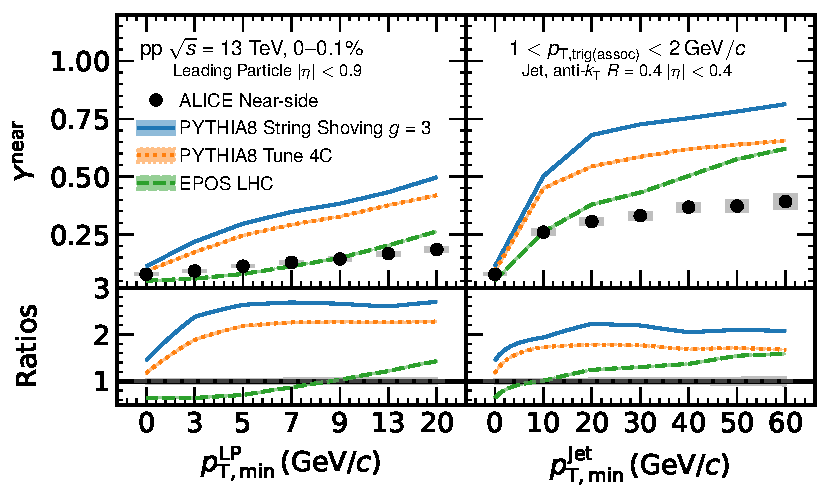
\includegraphics[width=0.89\linewidth]{./figures/Fig9_JetYieldESE.pdf}
	\caption{ Near-side jet-like peak yield with respect to the minimum leading particle(left) and jet selections(right). The filled circles show measurement with ALICE. The measurements are compared with model descriptions from $\pythiam$, $\pythiashoving$, and $\epos$ for both selections.}
	\label{fig:JetYield_ESE}
\end{figure}

Finally, Near-side jet-like peak yield was measured as a function of minimum $\ptlead$ and $\ptjet$ threshold in Fig.~\ref{fig:JetYield_ESE} to further test the models that aim to describe the near-side ridge.
%quantify the trend of the jet yield.
$\epos$ provides comparable estimates for near-side yields, while $\pythiam$ and $\pythiashoving$ overestimate near-side yields for both selections. Increasing trend of near-side yield as a function of minimum $\ptlead$ and saturating trend of near-side yield as a function of minimum $\ptjet$ have been observed, which are also qualitatively explained by models. Near-side jet-like peak yield measured with $\ptlead>$20~GeV/$c$ is comparable with the one measured with $\ptjet>$10~GeV/$c$, where ridge yields with corresponding selections are also comparable.